\section{Results and Analysis}
\label{sec:results-analysis}

% \textcolor{red}{This section should present the obtained results and provide an insightful analysis of them. You can present the results using graphs, tables, or any other visualization method suits your purpose. Do not forget to include proper captions \cite{zobel2014graphs} in any of these illustration methods you use. You do not need to provide any execution details as they are already presented in Sec.~\ref{sec:experimentation}.}

% \textcolor{red}{A good practise would be to compare your algorithm with a simpler approach, such as (a) a naive method, (b) a Hill Climbing approach, or (c) a simple evolutionary algorithm. In the third case, you can use the simpler version of the algorithm you developed, i.e., the original algorithm without your modifications. In that case, you should briefly describe the comparing method(s) in Sec.~\ref{sec:experimentation}. Alternatively, you can use some reference results derived from the repositories you found some benchmark instances.}

% \textcolor{red}{To display tables, the \texttt{booktabs} package might be useful. For example, Table~\ref{tab:results_example} shows how you should increase the  size of $n$, when running your code. You can advice \cite{zobel2014graphs} to see a few examples of proper tables.}

This chapter presents the performance of the GA on the boards of different complexities.

\subsection{Bayesian optimization results}

As mentioned in chapter \ref{sec:experimentation}, Bayesian Optimization is used to find the optimal population size and mutation rate for the GA. The results are shown in Figure~\ref{fig:bayesian_optimization_results}.

\subsubsection{Optimization progress}

Chart one of Figure~\ref{fig:bayesian_optimization_results} shows that the difference between the best and the worst score is minimal, meaning that the GA is stable and the hyperparameters are selected well.

\subsubsection{Population size vs Performance}

From chart two of Figure~\ref{fig:bayesian_optimization_results} we can see a population size of around 100 and 900 can find solutions in a shorter time while the score is more discrete at population size 900. Thus, the average time of solving puzzles at population size 900 is costlier than at population size 150.

\subsubsection{Mutation rate vs Performance}

Chart three of Figure~\ref{fig:bayesian_optimization_results} presents that the mutation rate between 0.05 and 0.15 could often times not find a solution. When mutation rate reaches over 0.20, the number of failure cases decreased and no solution events happened less frequently.

\subsubsection{Parameter space exploration}

Chart four of Figure~\ref{fig:bayesian_optimization_results} shows that the best population size is 142 and the best mutation rate is 0.230. This result is based on the best score shown in the first chart.

\begin{figure}[H]
\centering
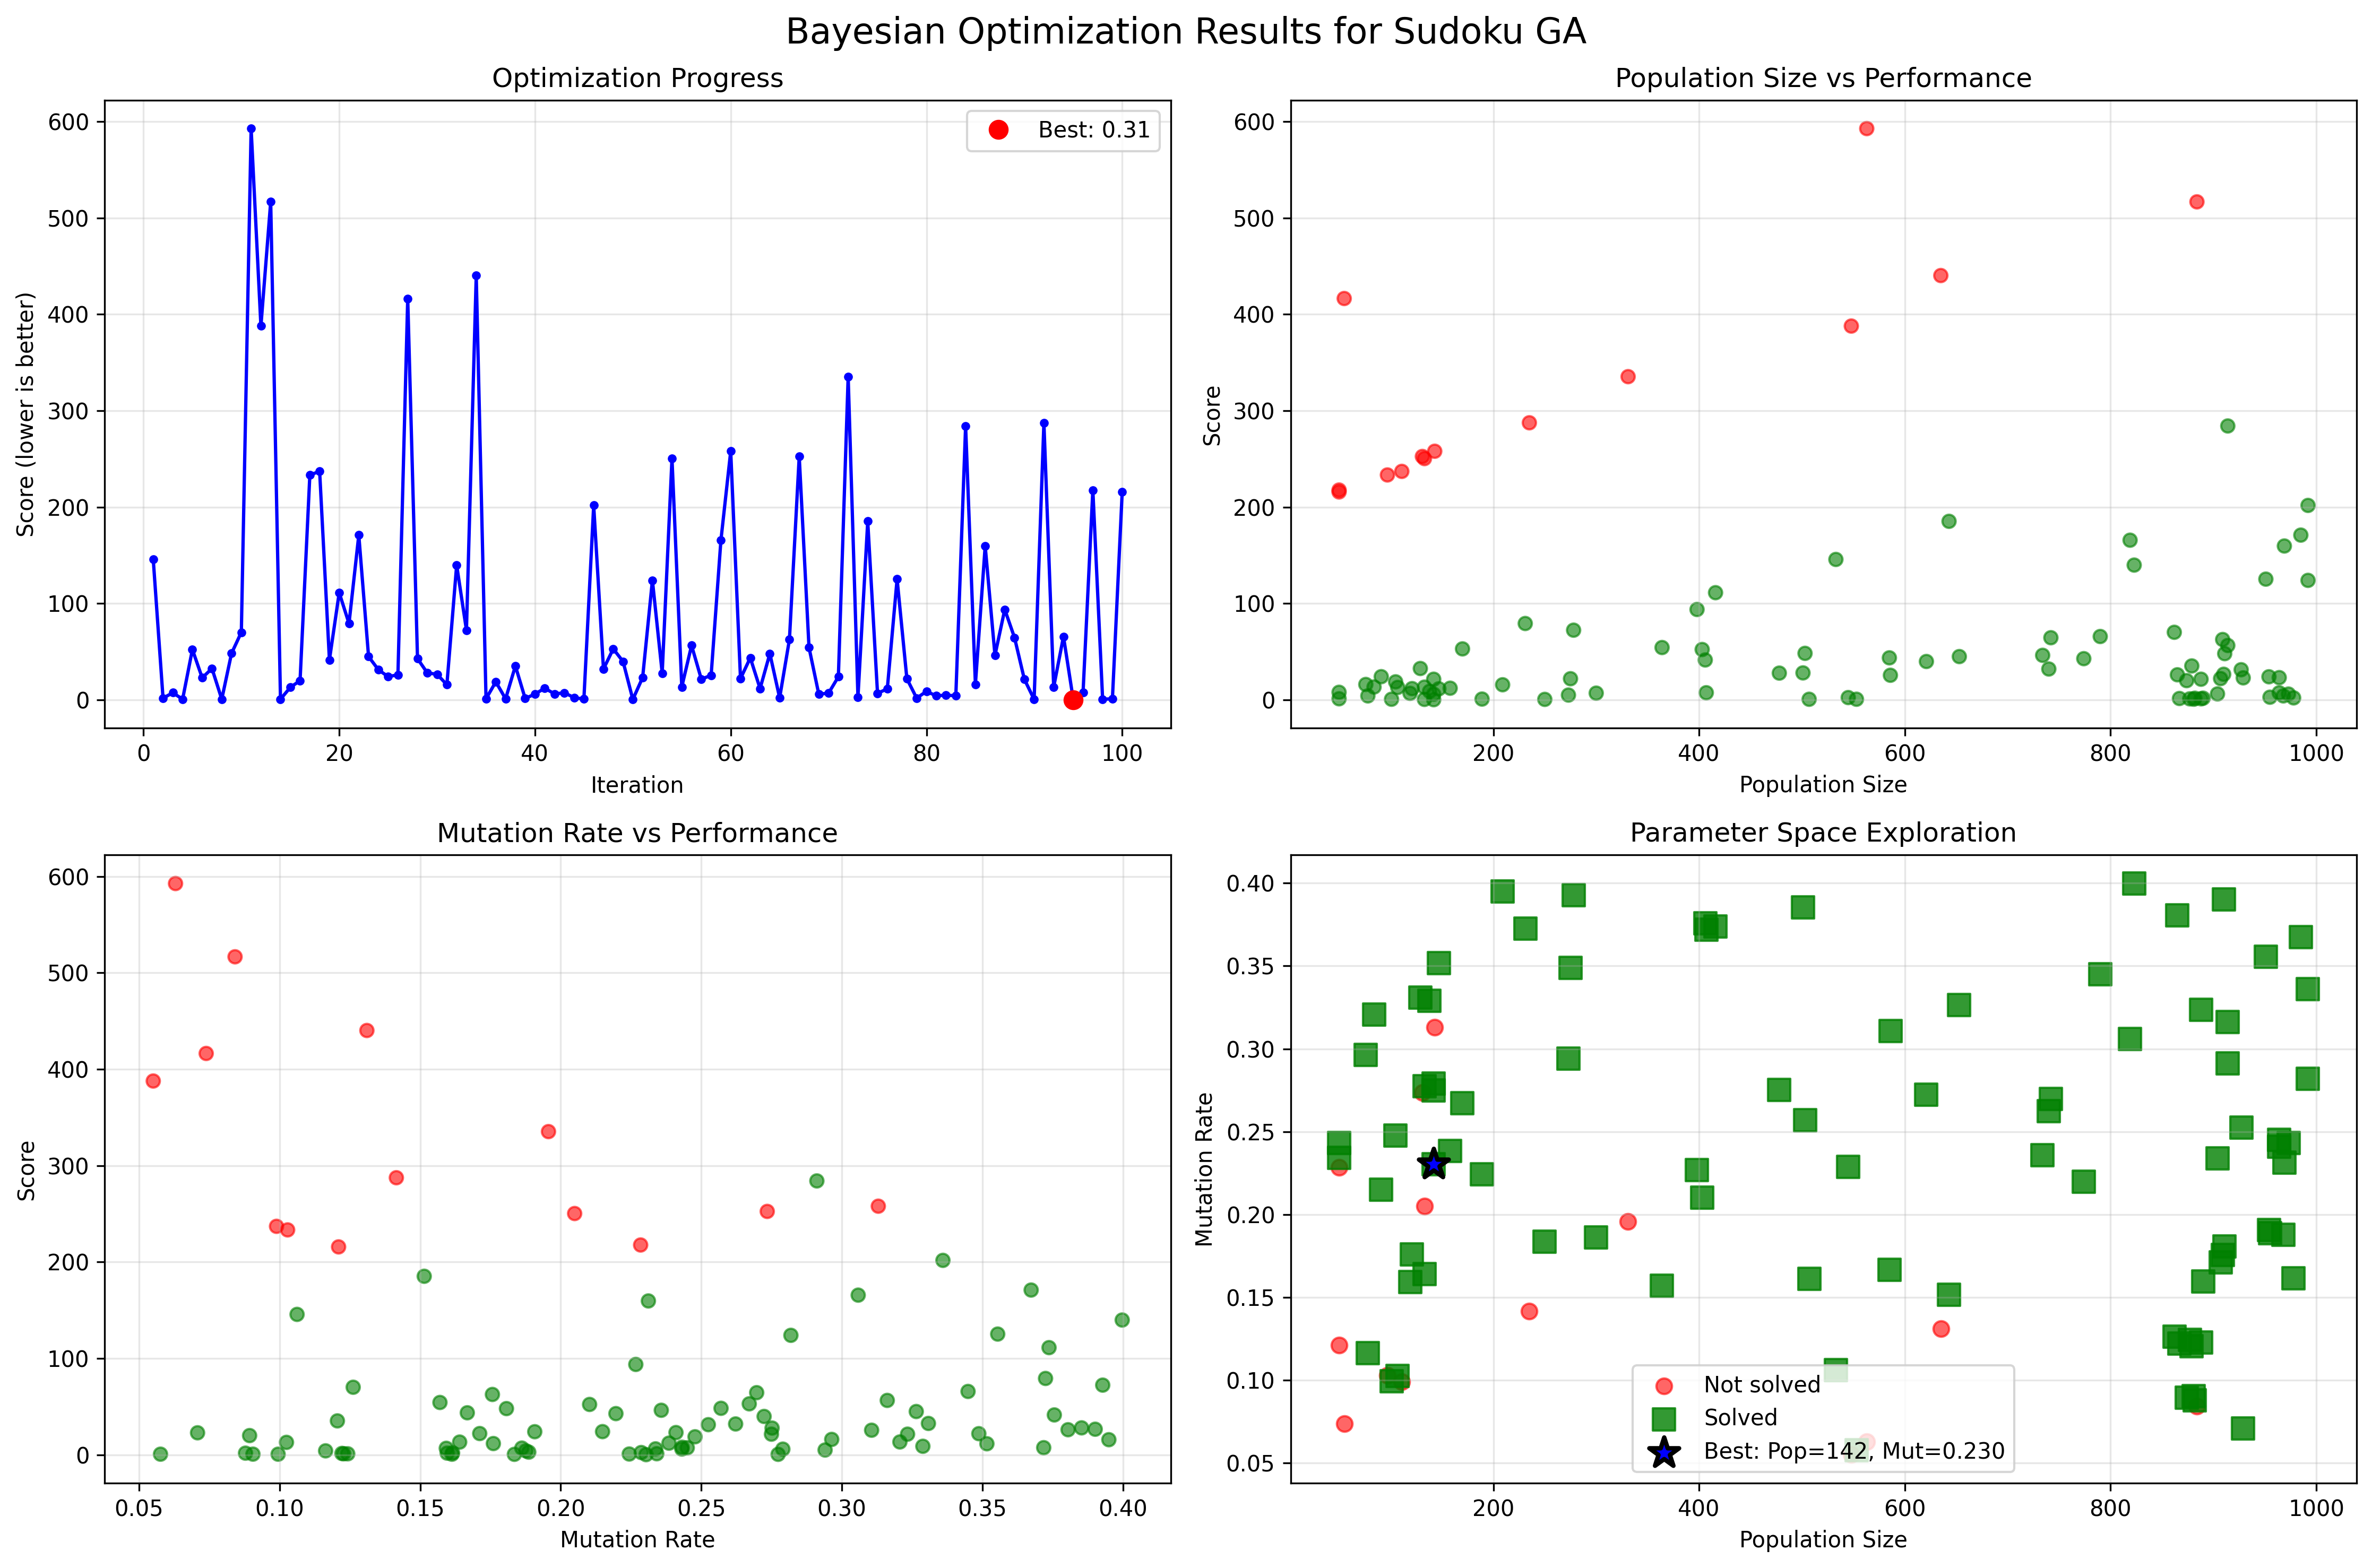
\includegraphics[width=0.8\textwidth]{resources/bayesian_optimization_results.png}
\caption{Bayesian optimization results.}
\label{fig:bayesian_optimization_results}
\end{figure}

\subsection{Performance of the GA}

We test easy, medium and hard difficulty puzzles in the same setting, but as mentioned in chapter \ref{sec:experimentation} it is costly to test each difficulty 1000 times. Thus, we only test the easy difficulty for 1000 times, the medium one for around 400 times, and the hard one for 100 times.

\subsubsection{Easy difficulty}

The charts below shows the performance of the GA with easy difficulty puzzles. For every single board a solution was found by the GA. In over 500 times we find a solution in less than 0.5 seconds. Only around \(\frac{1}{20}\) of the solutions are reached very slow which is more than 20s.
Additionally, the average execution time is 5s, which is a good performance. Moreover, the execution time and generation have linear relationship which means that if the algorithm needs more generations to find the solution, the more execution time it will cost.

\begin{figure}[H]
\centering
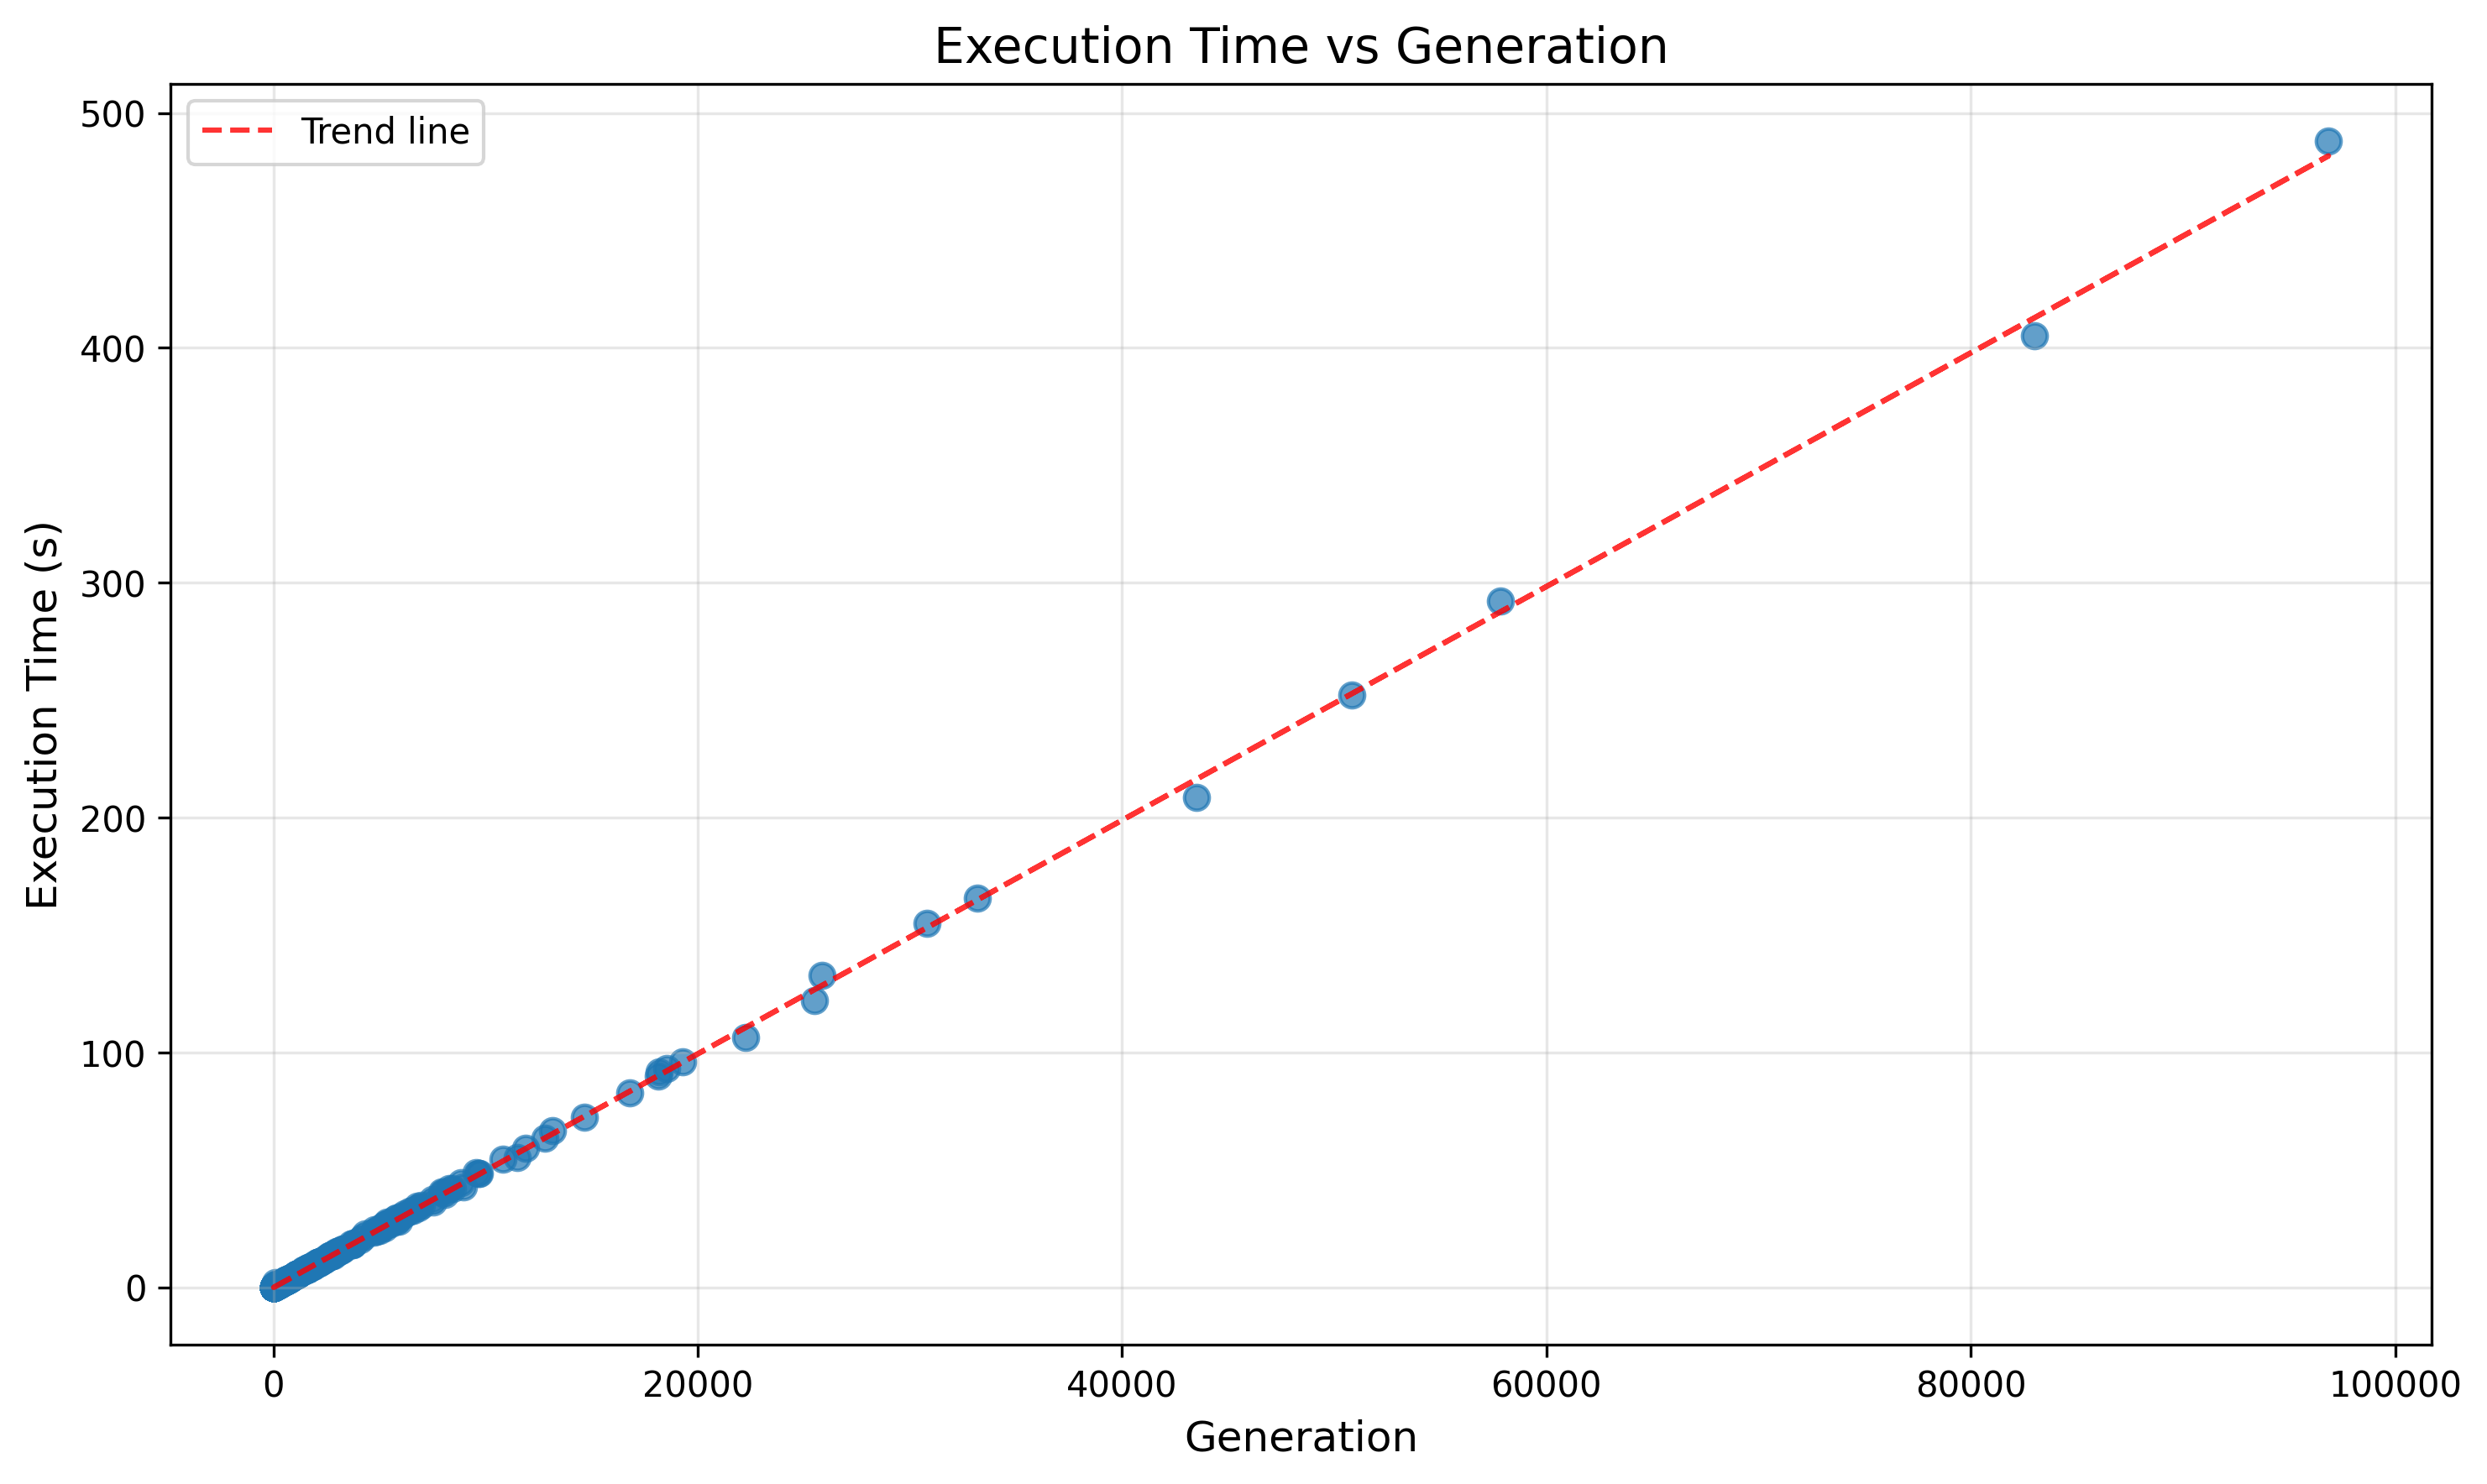
\includegraphics[width=0.8\textwidth]{resources/generation_vs_execution_time_easy.png}
\caption{Generation vs execution time for easy difficulty puzzles.}
\label{fig:generation_vs_execution_time_easy}
\end{figure}

\begin{figure}[H]
\centering
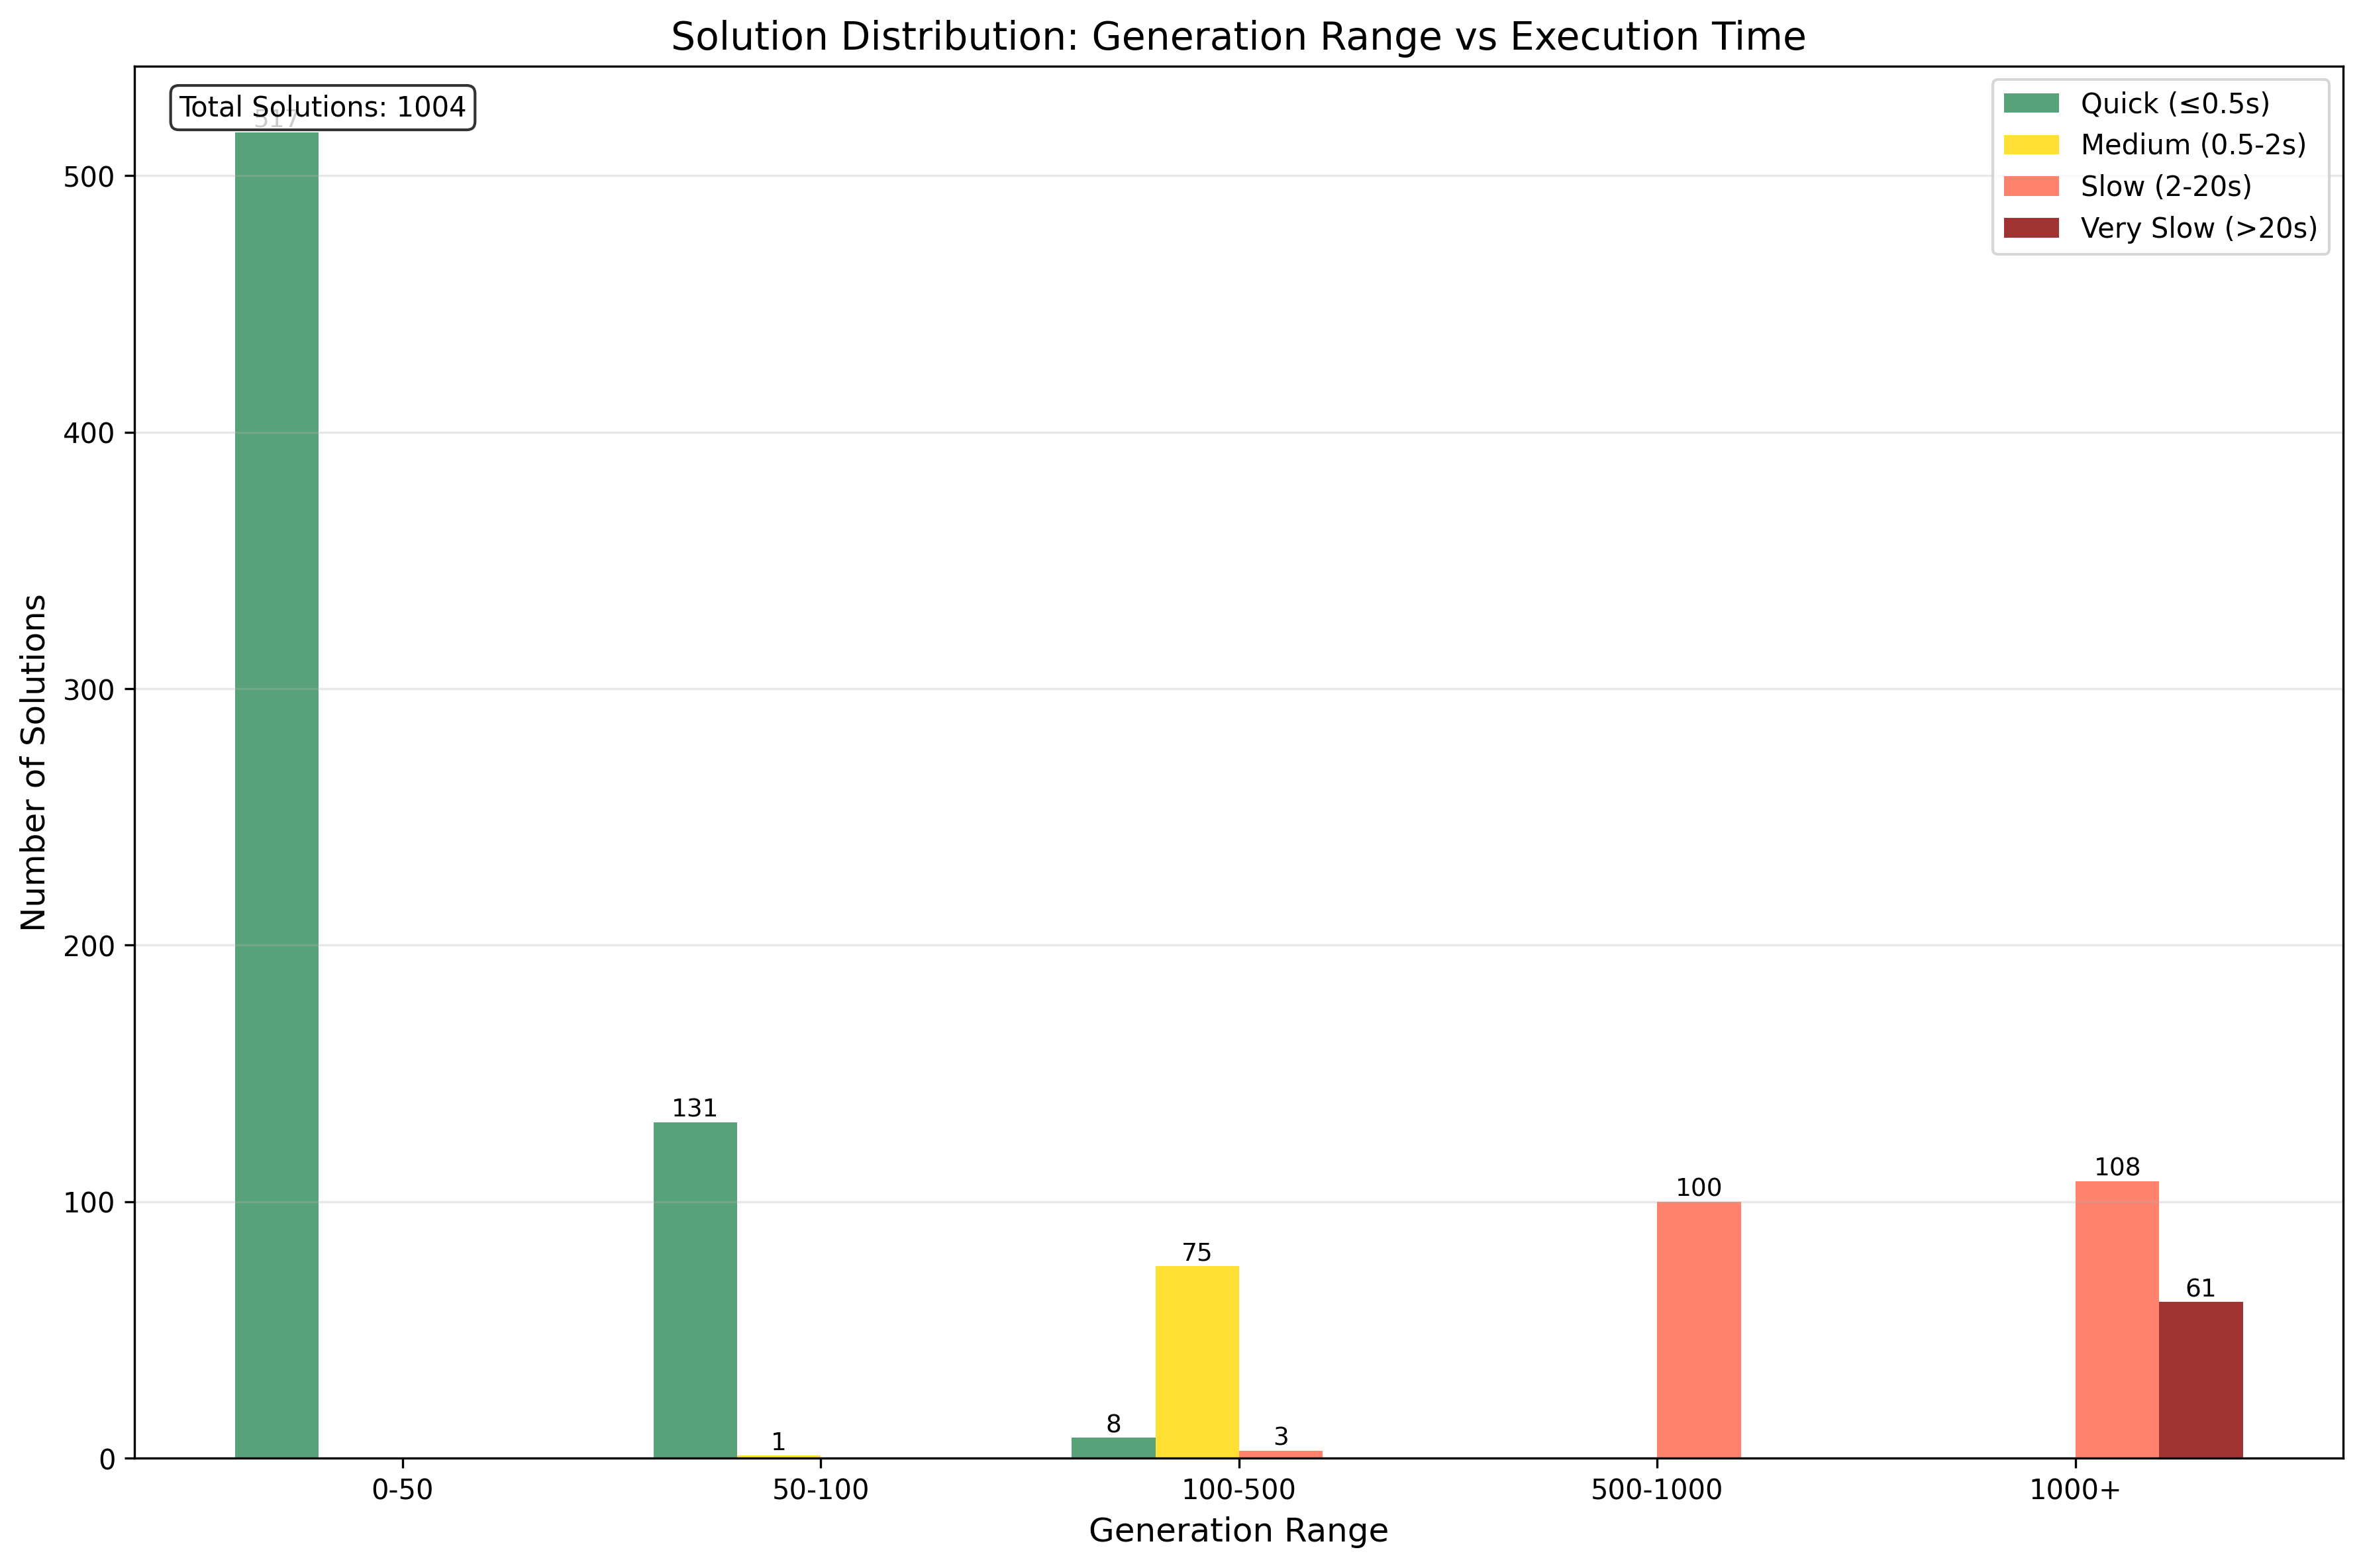
\includegraphics[width=0.8\textwidth]{resources/generation_execution_time_bars_easy.png}
\caption{Generation and execution time distribution for easy difficulty puzzles.}
\label{fig:generation_execution_time_bars_easy}
\end{figure}

\paragraph{Easy Difficulty Statistical Analysis}

Table~\ref{tab:easy_difficulty_stats} presents a comprehensive statistical analysis of the genetic algorithm performance on easy difficulty Sudoku puzzles over 1000 runs.

\begin{table}[H]
\centering
\caption{Statistical Analysis of GA Performance on Easy Difficulty Puzzles}
\label{tab:easy_difficulty_stats}
\begin{tabular}{@{}lc@{}}
\toprule
\textbf{Metric} & \textbf{Value} \\
\midrule
Total Runs & 1000 \\
Successful Runs & 1000 (100\%) \\
Failed Runs & 0 (0\%) \\
\midrule
\textbf{Execution Time} & \\
Average & 5.99s \\
Range & 0.03s -- 488.11s\\
Successful Runs (Avg) & 5.99s \\
Failed Runs (Avg) & 0s \\
\midrule
\textbf{Generations} & \\
Average & 1202.4 \\
Range & 6 -- 96862 \\
Generations per Second & 204.55 \\
\midrule
\textbf{Solution Quality} & \\
Average Violations & 0.0 \\
Failed Runs Violations & 0 (constant) \\
\bottomrule
\end{tabular}
\end{table}

\subsubsection{Medium difficulty}

The charts below shows the performance of the GA with medium difficulty. At 91,4\%, a solution for most of the boards could be found. The time cost of finding a solution at quick and medium time only plays a small role in the total cases.
Additionally, the proportion of the getting solution in very slow is $60\%$, which is much higher compared to easy difficulty.
Meanwhile, the execution time and generation still remain a linear relationship.

\begin{figure}[H]
\centering
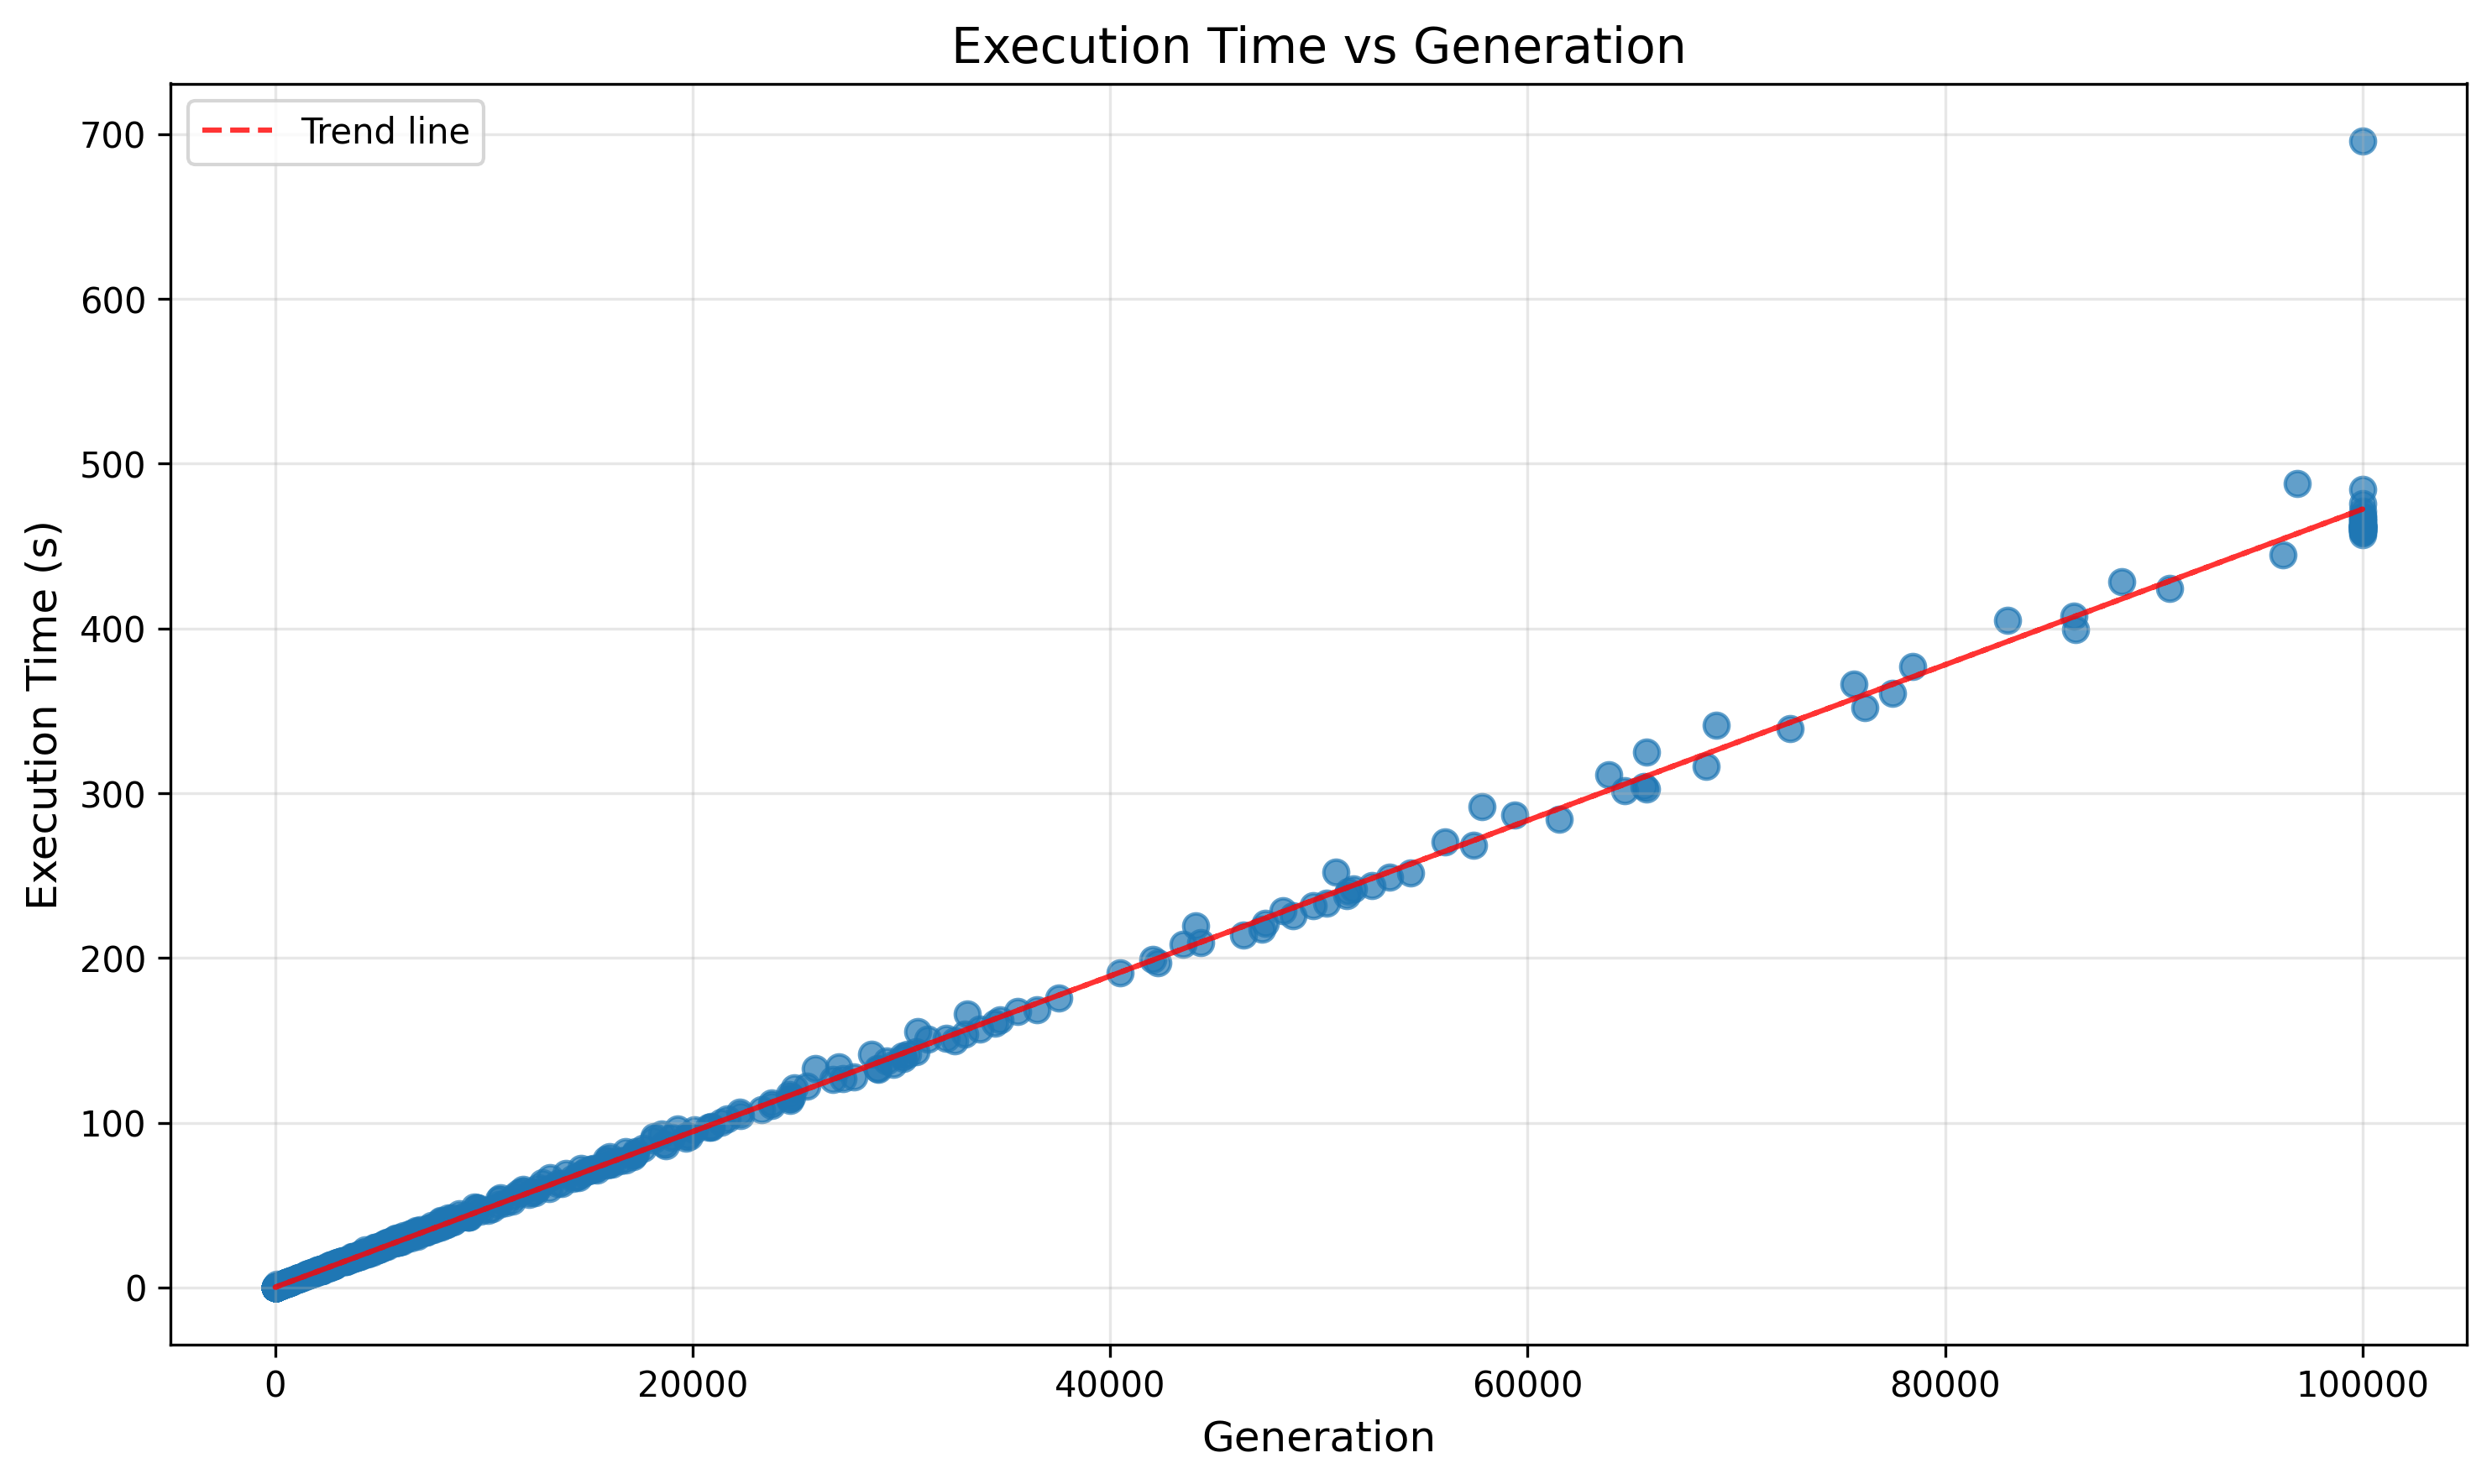
\includegraphics[width=0.8\textwidth]{resources/generation_vs_execution_time_medium.png}
\caption{Generation vs execution time for medium difficulty puzzles.}
\label{fig:generation_vs_execution_time_medium}
\end{figure}

\begin{figure}[H]
\centering
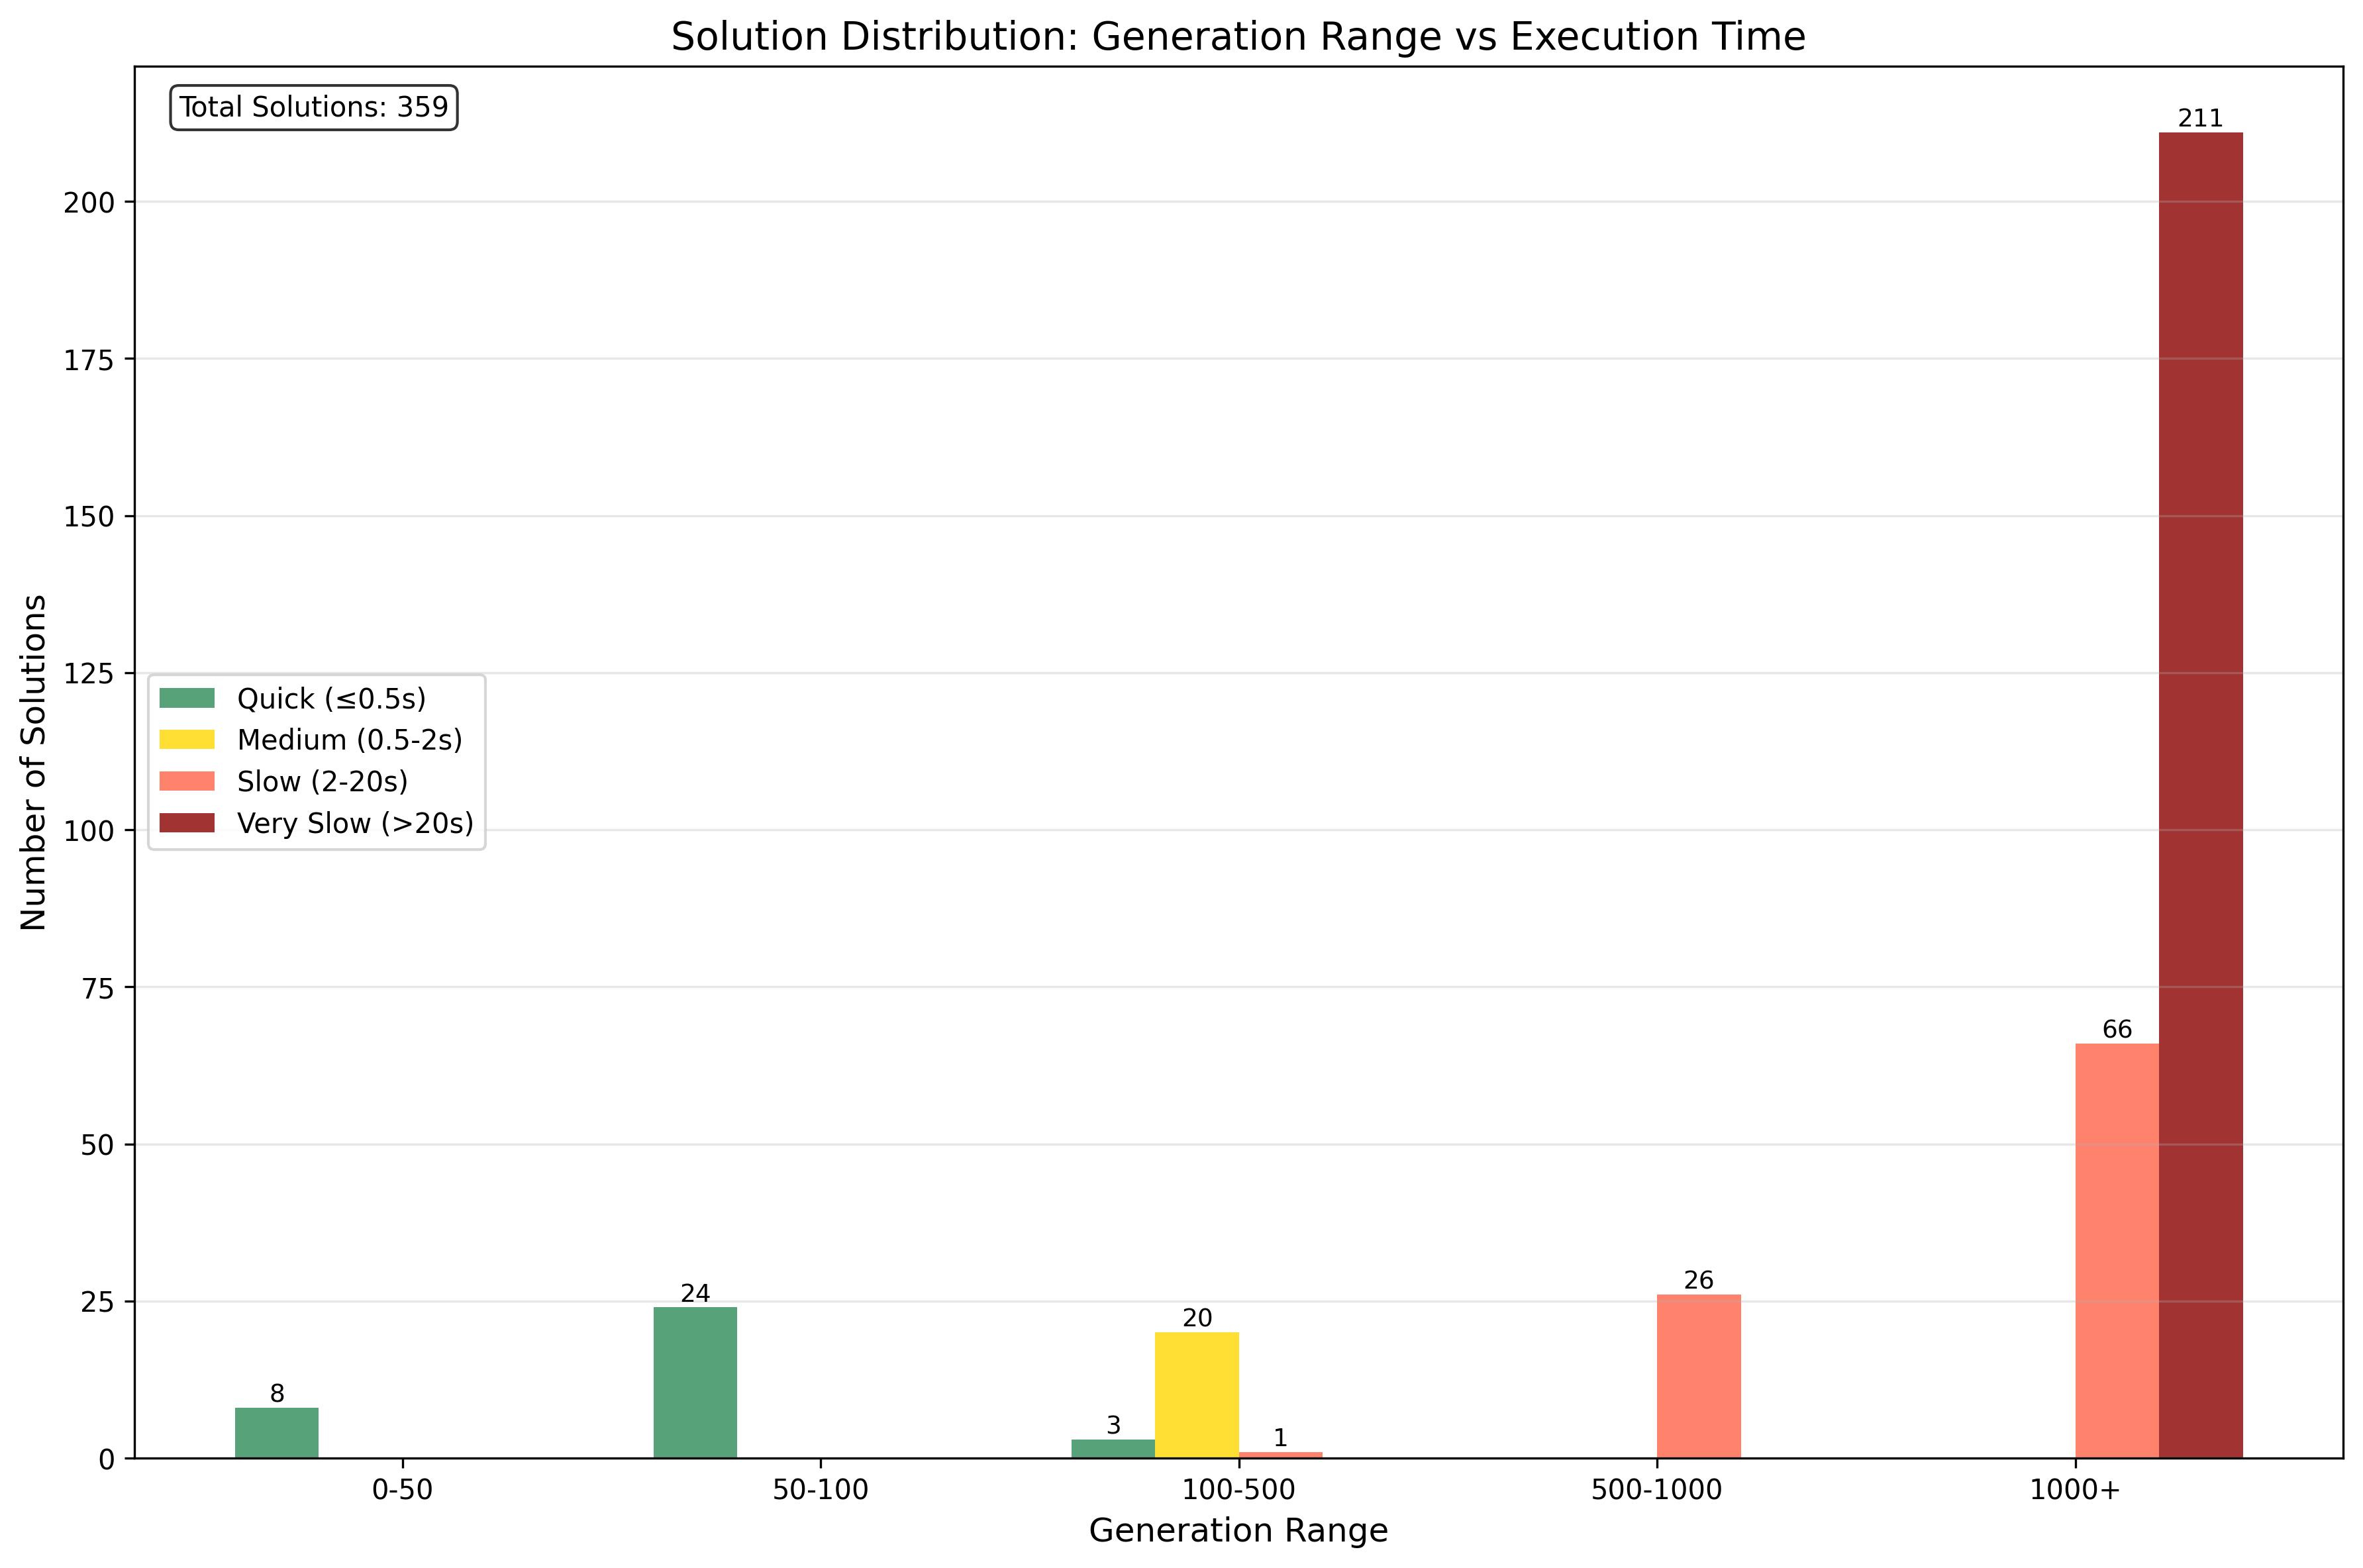
\includegraphics[width=0.8\textwidth]{resources/generation_execution_time_bars_medium.png}
\caption{Generation and execution time distribution for medium difficulty puzzles.}
\label{fig:generation_execution_time_bars_medium}
\end{figure}

\paragraph{Medium Difficulty Statistical Analysis}

Table~\ref{tab:medium_difficulty_stats} presents a comprehensive statistical analysis of the genetic algorithm performance on medium difficulty Sudoku puzzles over 300 runs.

\begin{table}[H]
\centering
\caption{Statistical Analysis of GA Performance on Medium Difficulty Puzzles}
\label{tab:medium_difficulty_stats}
\begin{tabular}{@{}lc@{}}
\toprule
\textbf{Metric} & \textbf{Value} \\
\midrule
Total Runs & 359 \\
Successful Runs & 328 (91.4\%) \\
Failed Runs & 31 (8.6\%) \\
\midrule
\textbf{Execution Time} & \\
Average & 102.05s \\
Range & 0.13s -- 695.95s \\
Successful Runs (Avg) & 67.17s \\
Failed Runs (Avg) & 471.15s \\
\midrule
\textbf{Generations} & \\
Average & 21681.9 \\
Range & 30 -- 100,000 \\
Generations per Second & 213.95 \\
\midrule
\textbf{Solution Quality} & \\
Average Violations & 0.2 \\
Failed Runs Violations & 2.0 (constant) \\
\bottomrule
\end{tabular}
\end{table}

\subsubsection{Hard difficulty}

The charts below shows the performance of the GA with hard difficulty. The number of solutions found decreased drastically. Only 45\% of boards could be solved. The proportion of getting the solution in very slow is $97\%$ which is much higher compared to easy and medium difficulty.
Meanwhile, the execution time and generation still remain a linear relationship.

\begin{figure}[H]
\centering
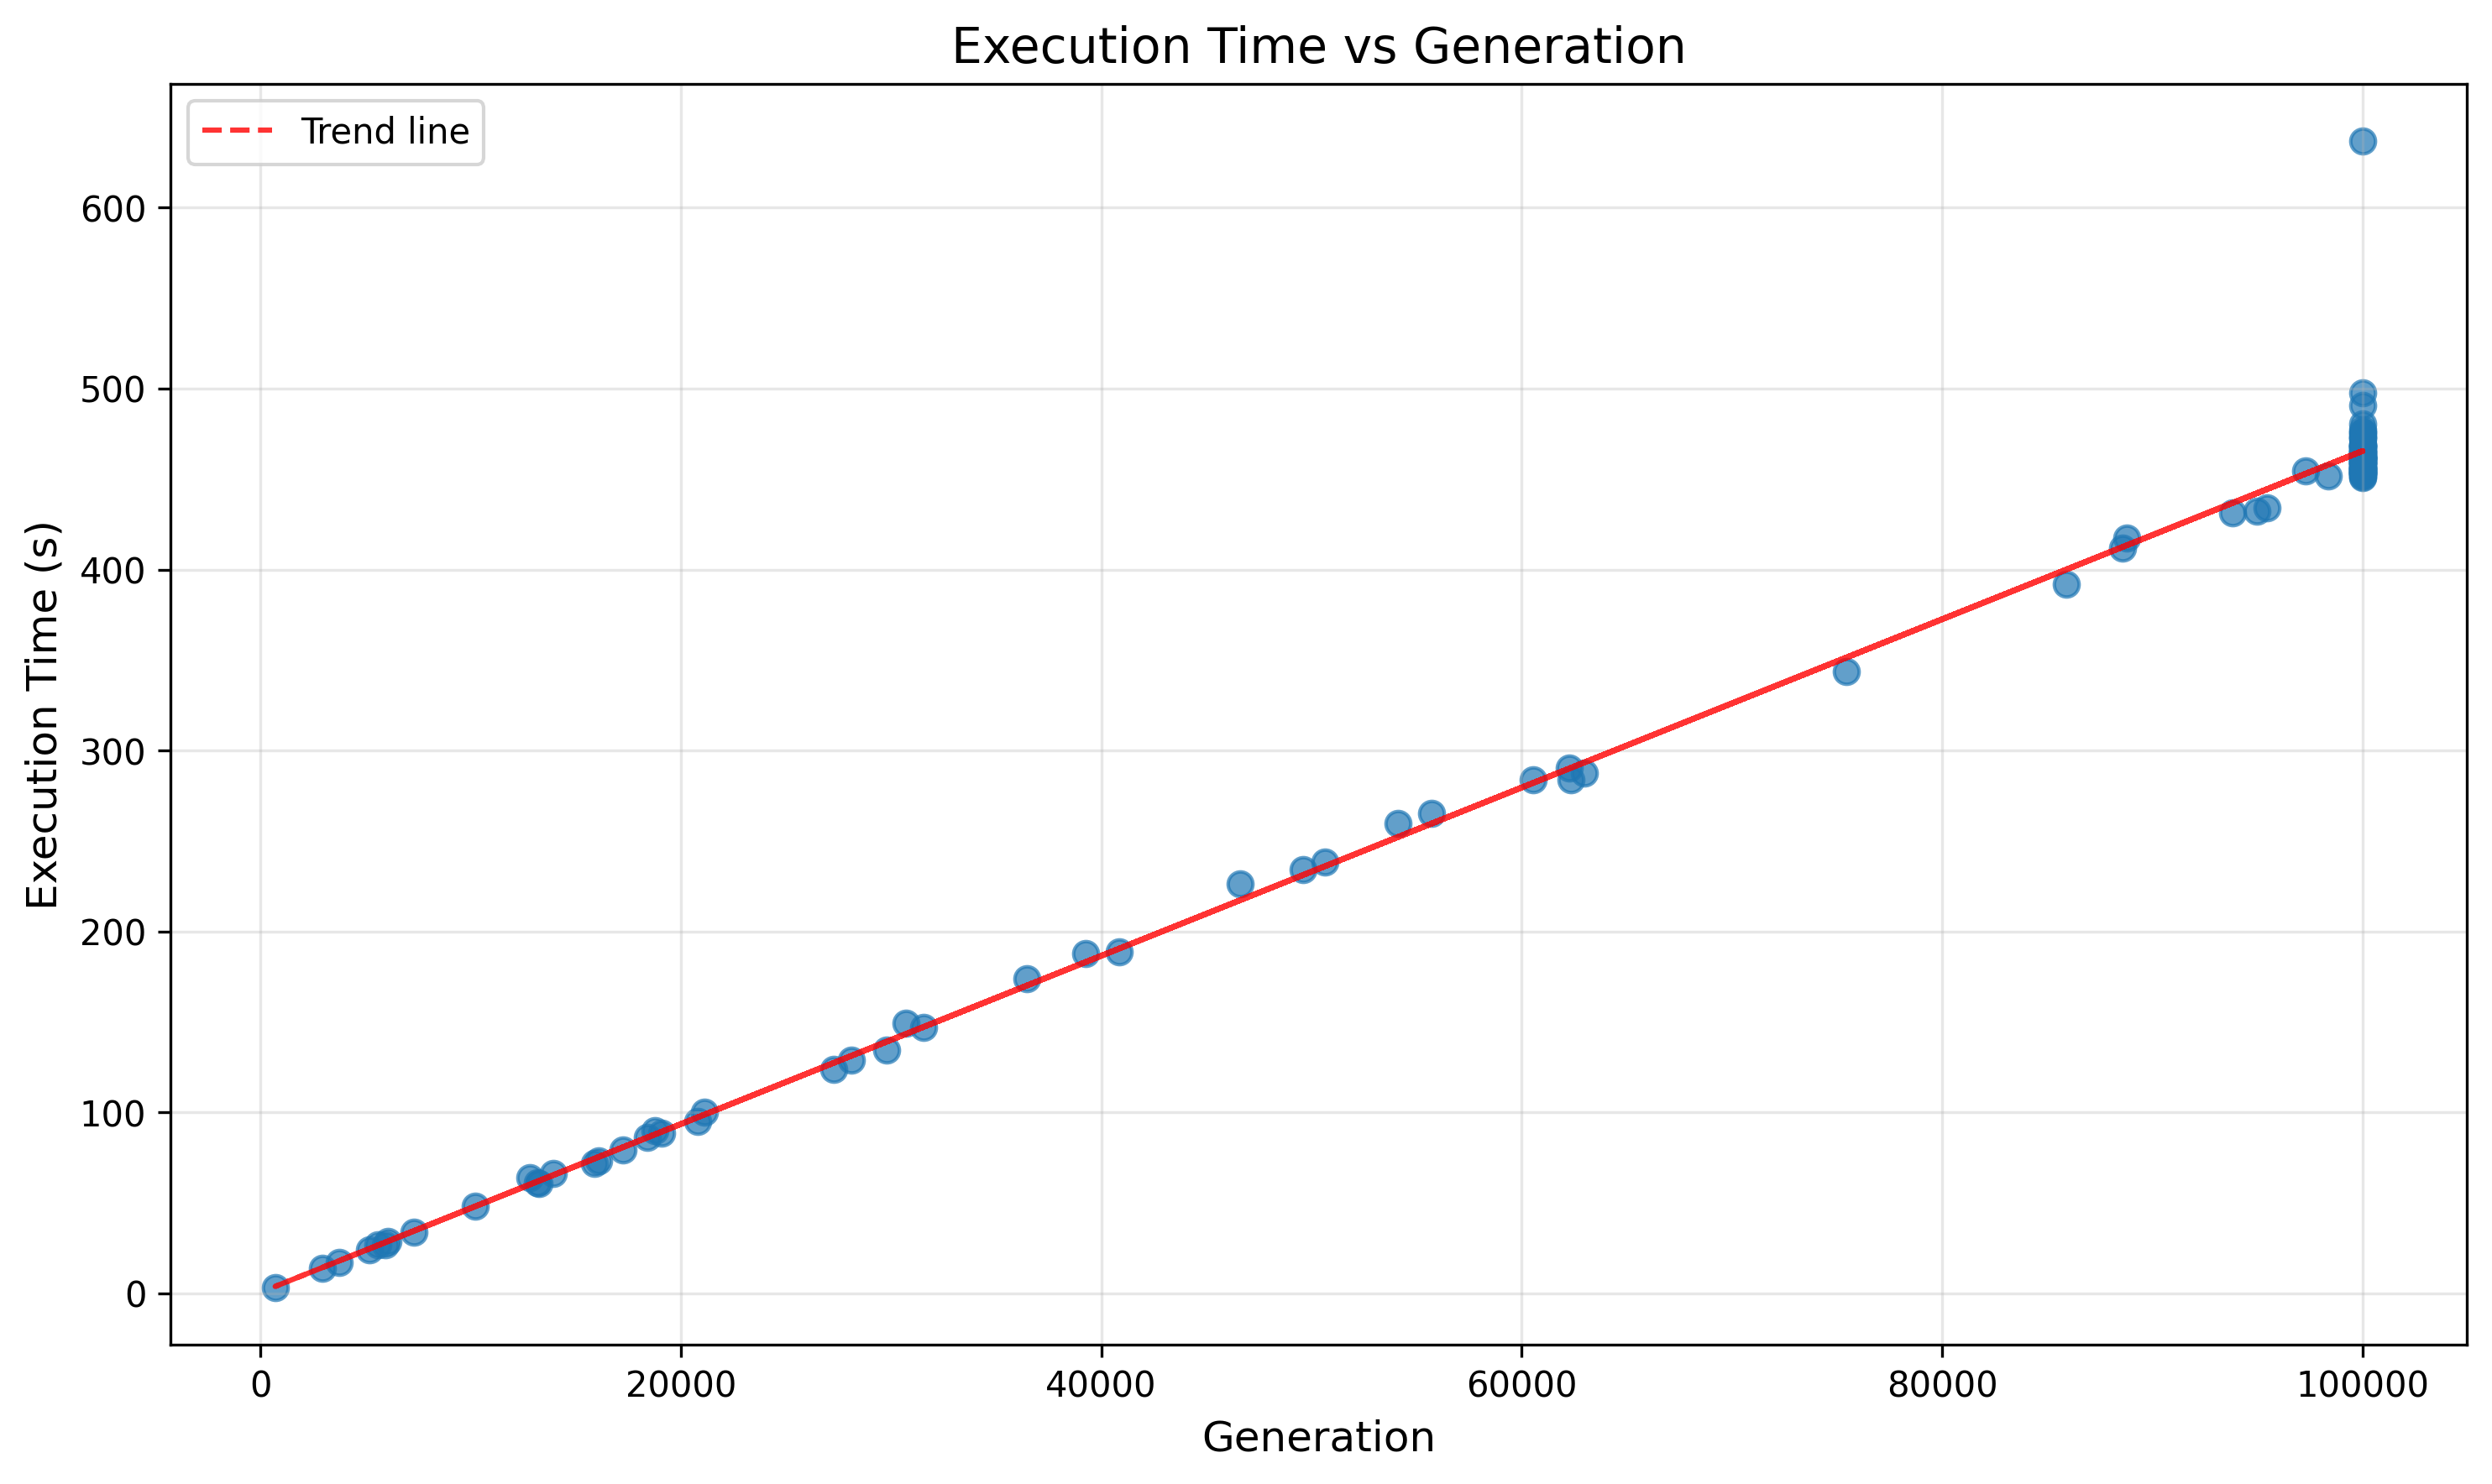
\includegraphics[width=0.8\textwidth]{resources/generation_vs_execution_time_hard.png}
\caption{Generation vs execution time for hard difficulty puzzles.}
\label{fig:generation_vs_execution_time_hard}
\end{figure}

\begin{figure}[H]
\centering
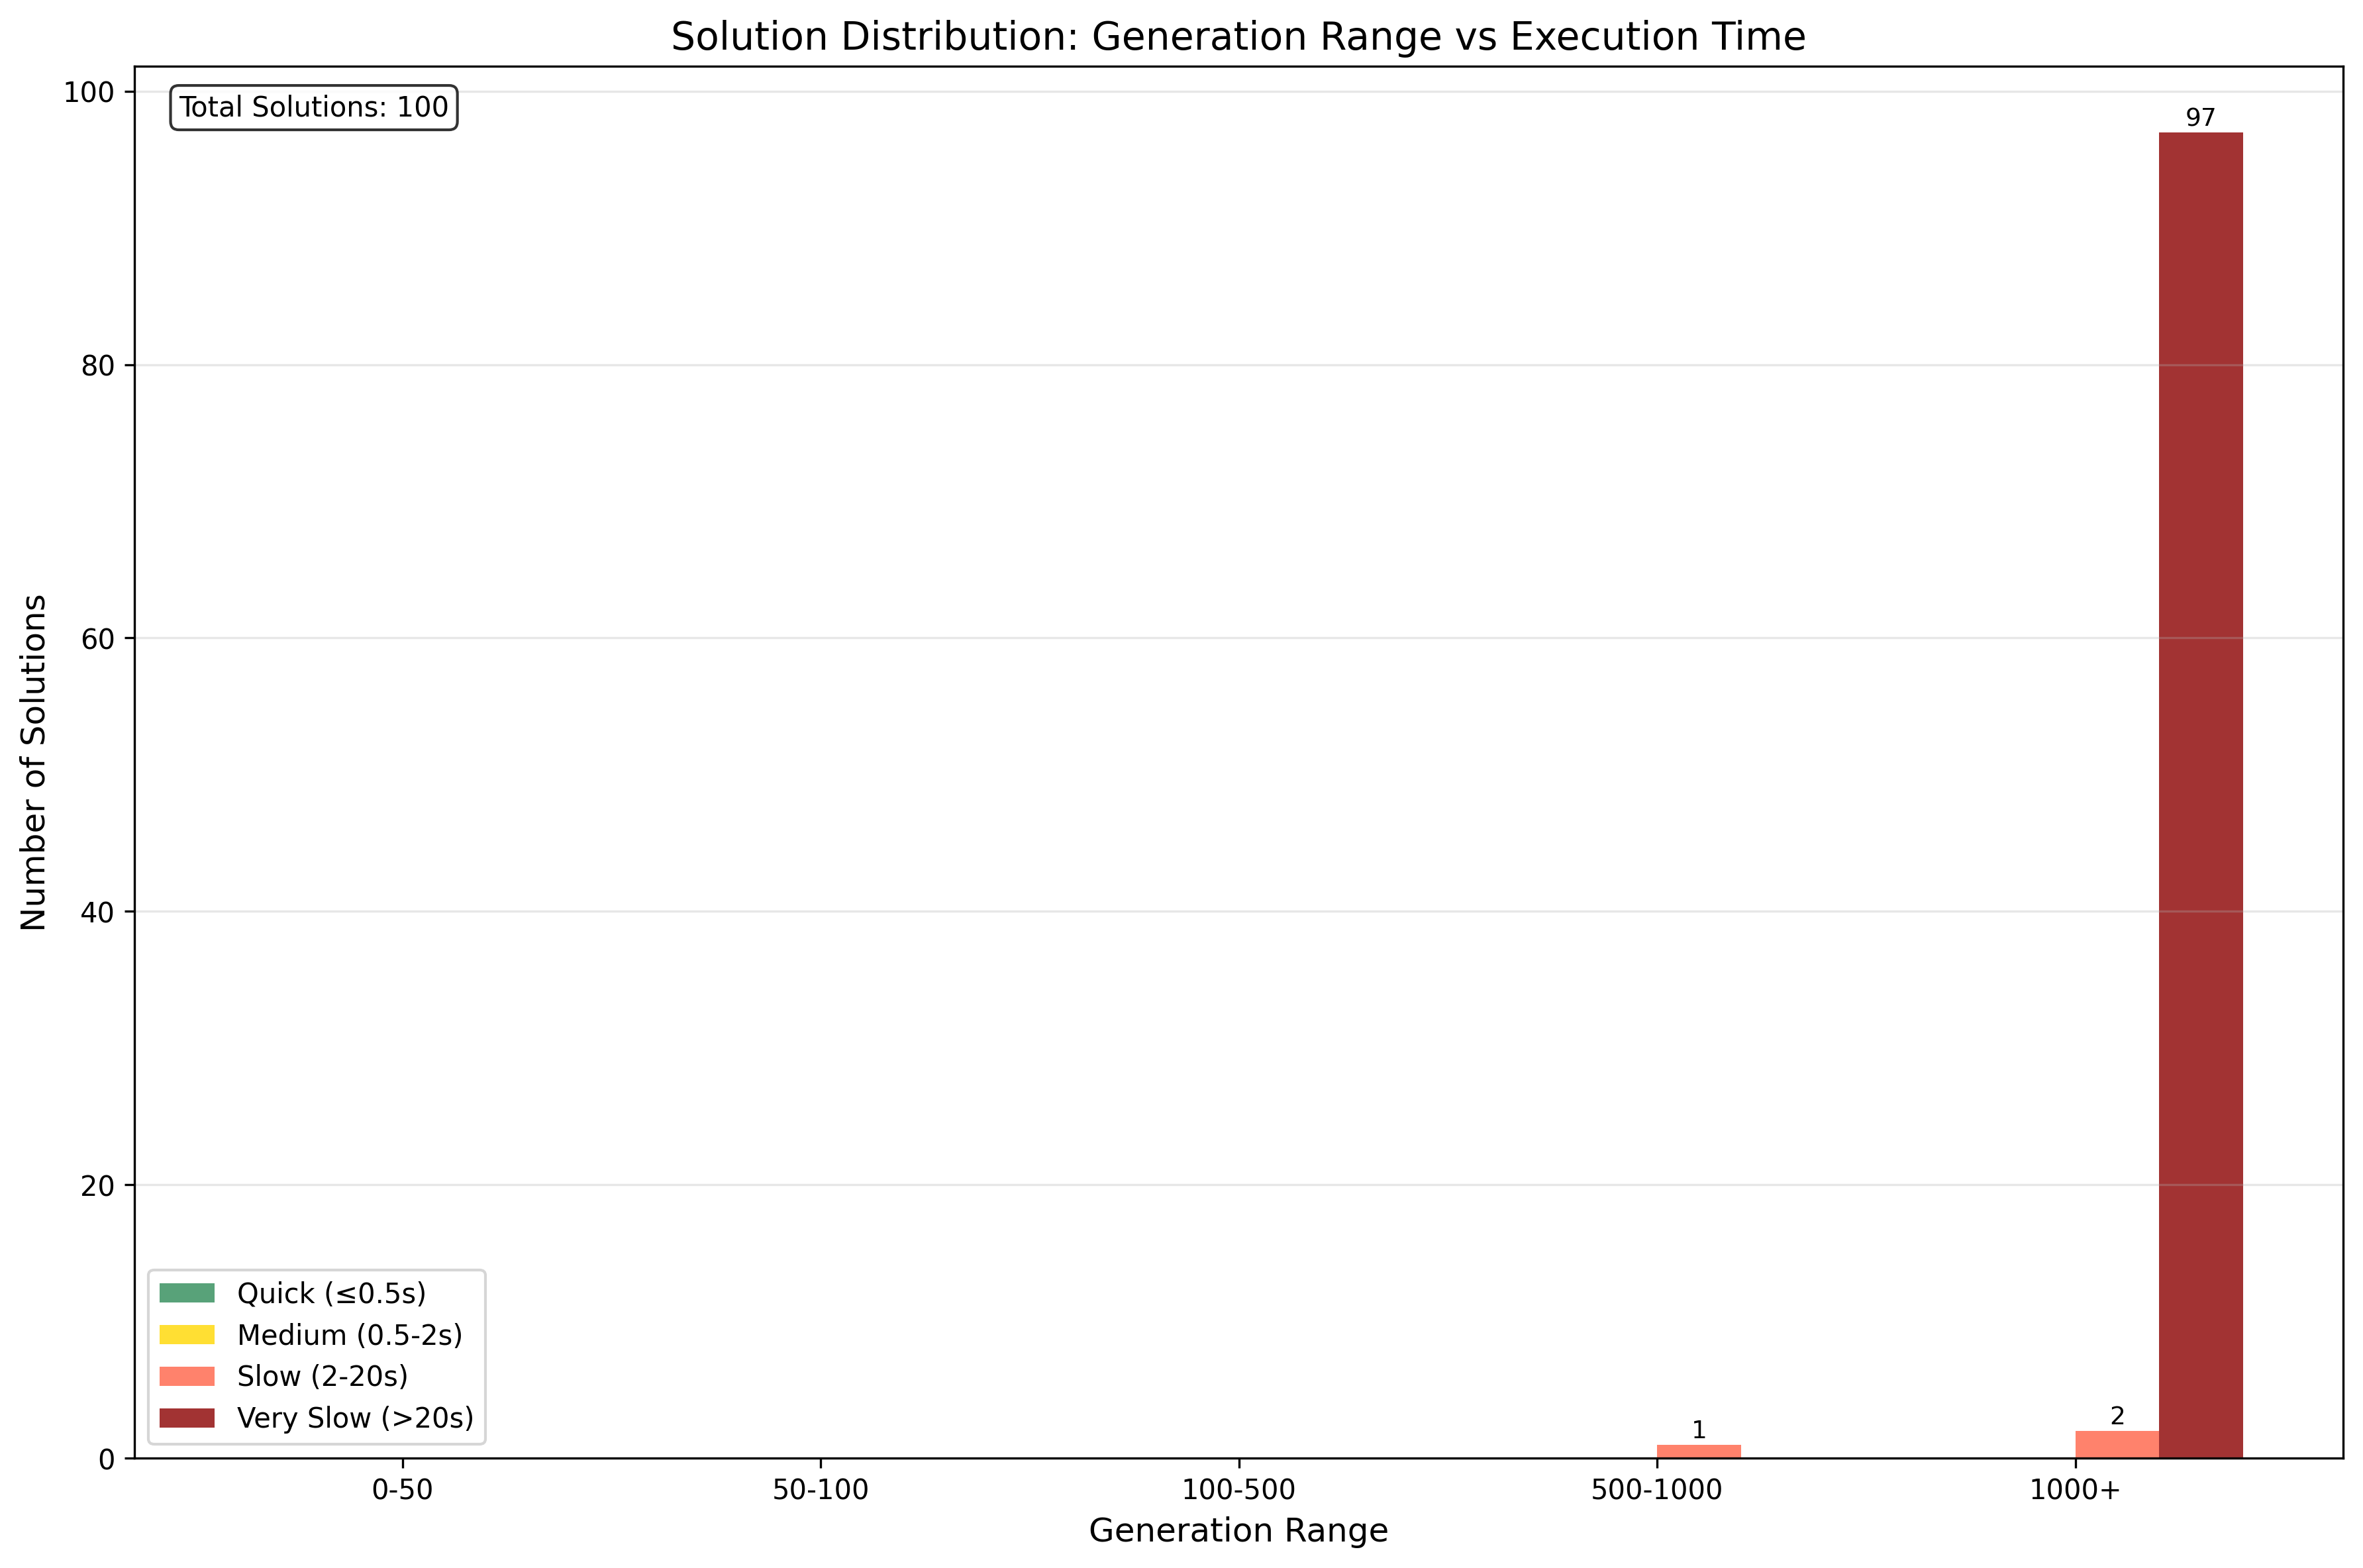
\includegraphics[width=0.8\textwidth]{resources/generation_execution_time_bars_hard.png}
\caption{Generation and execution time distribution for hard difficulty puzzles.}
\label{fig:generation_execution_time_bars_hard}
\end{figure}

\paragraph{Hard Difficulty Statistical Analysis}

Table~\ref{tab:hard_difficulty_stats} presents a comprehensive statistical analysis of the genetic algorithm performance on hard difficulty Sudoku puzzles over 100 runs.

\begin{table}[H]
\centering
\caption{Statistical Analysis of GA Performance on Hard Difficulty Puzzles}
\label{tab:hard_difficulty_stats}
\begin{tabular}{@{}lc@{}}
\toprule
\textbf{Metric} & \textbf{Value} \\
\midrule
Total Runs & 100 \\
Successful Runs & 45 (45.0\%) \\
Failed Runs & 55 (55.0\%) \\
\midrule
\textbf{Execution Time} & \\
Average & 338.62s \\
Range & 3.22s -- 636.92s \\
Successful Runs (Avg) & 183.11s \\
Failed Runs (Avg) & 465.85s \\
\midrule
\textbf{Generations} & \\
Average & 72,763.8 \\
Range & 705 -- 100,000 \\
Generations per Second & 215.18 \\
\midrule
\textbf{Solution Quality} & \\
Average Violations & 1.1 \\
Failed Runs Violations & 2.0 (constant) \\
\bottomrule
\end{tabular}
\end{table}

\subsubsection{Performance Analysis}
The results reveal significant challenges as difficulty increases the performance of the GA:
\begin{itemize}
    \item The success rate decreases to 45\% on the hard level, compared with 100\% on the easy level and 91.4\% on the medium level, which reflects the higher complexity of hard puzzles.
    \item Failed runs take 282.75s longer on average than successful runs (465.85s vs 183.11s) on hard level. However, the average successful run time compared with failed runs (67.17s vs 471.15s).
    \item All failed runs (100\%) were stuck at local minima with exactly 2 violations
    \item Average of 85,181 generations without improvement in failed runs which is better than the medium level (91661.1).
\end{itemize}

\subsection{Performance of DFS}

We test the performace of the rule based algorithm with easy, medium and hard difficulty.

\begin{figure}[H]
\centering
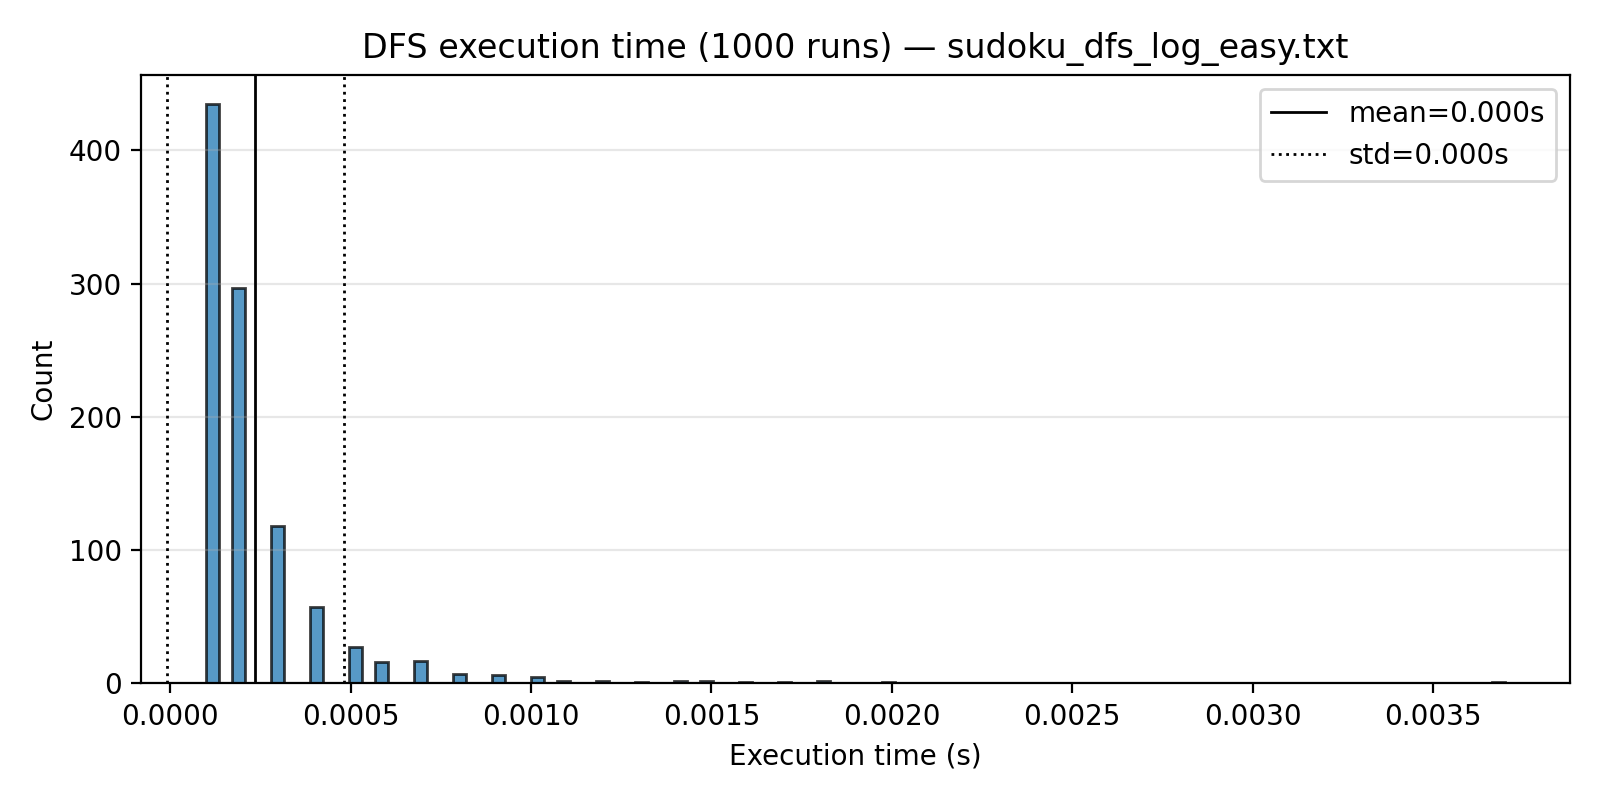
\includegraphics[width=0.8\textwidth]{resources/sudoku_dfs_log_easy_histogram.png}
\caption{sudoku\_dfs\_log\_easy\_histogram.}
\label{fig:sudoku_dfs_log_easy_histogram}
\end{figure}

\begin{figure}[H]
\centering
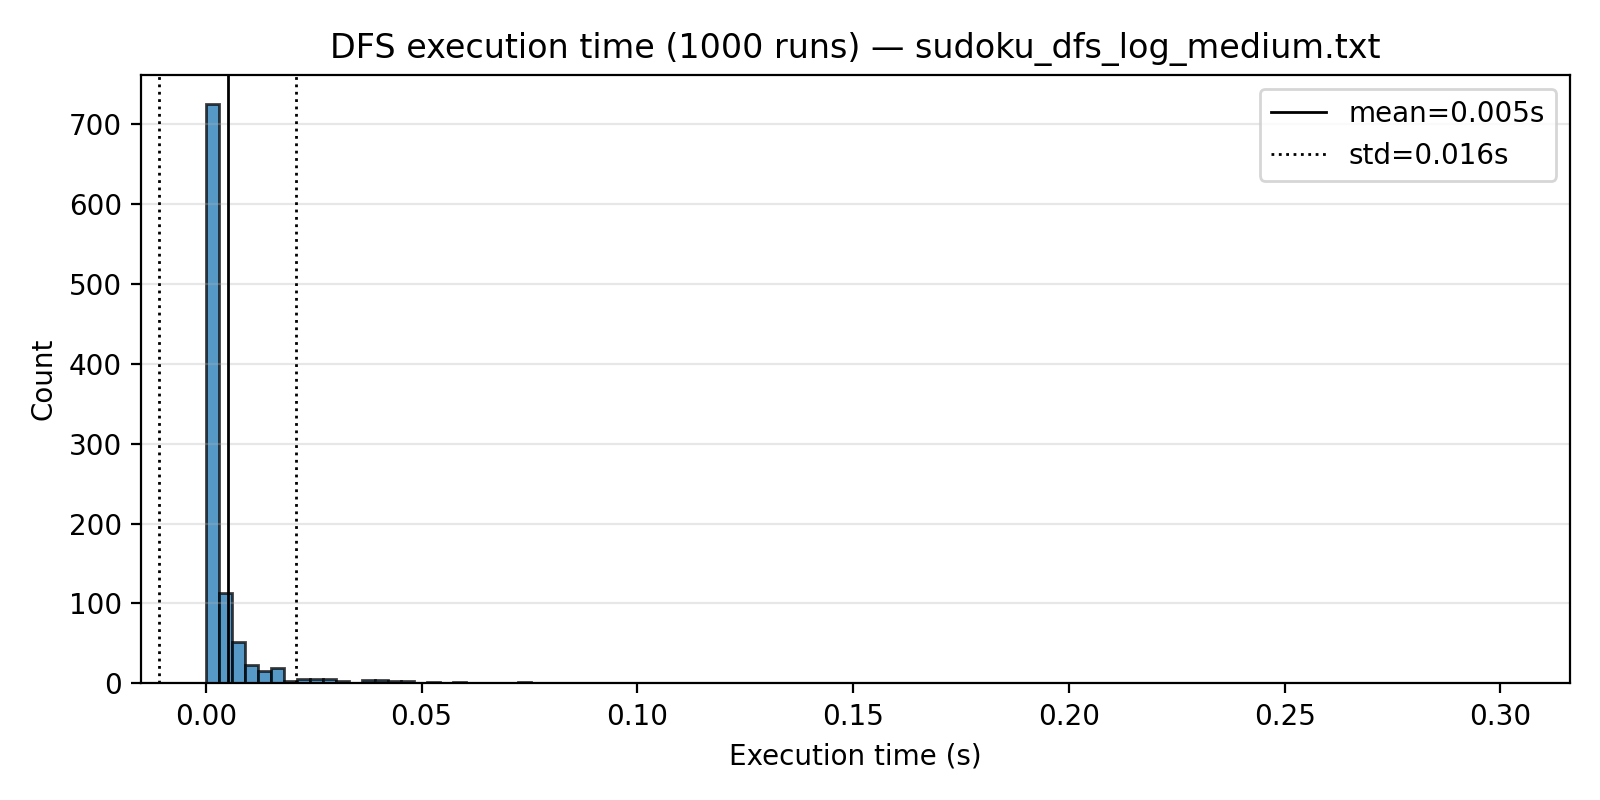
\includegraphics[width=0.8\textwidth]{resources/sudoku_dfs_log_medium_histogram.png}
\caption{sudoku\_dfs\_log\_medium\_histogram.}
\label{fig:sudoku_dfs_log_medium_histogram}
\end{figure}

\begin{figure}[H]
\centering
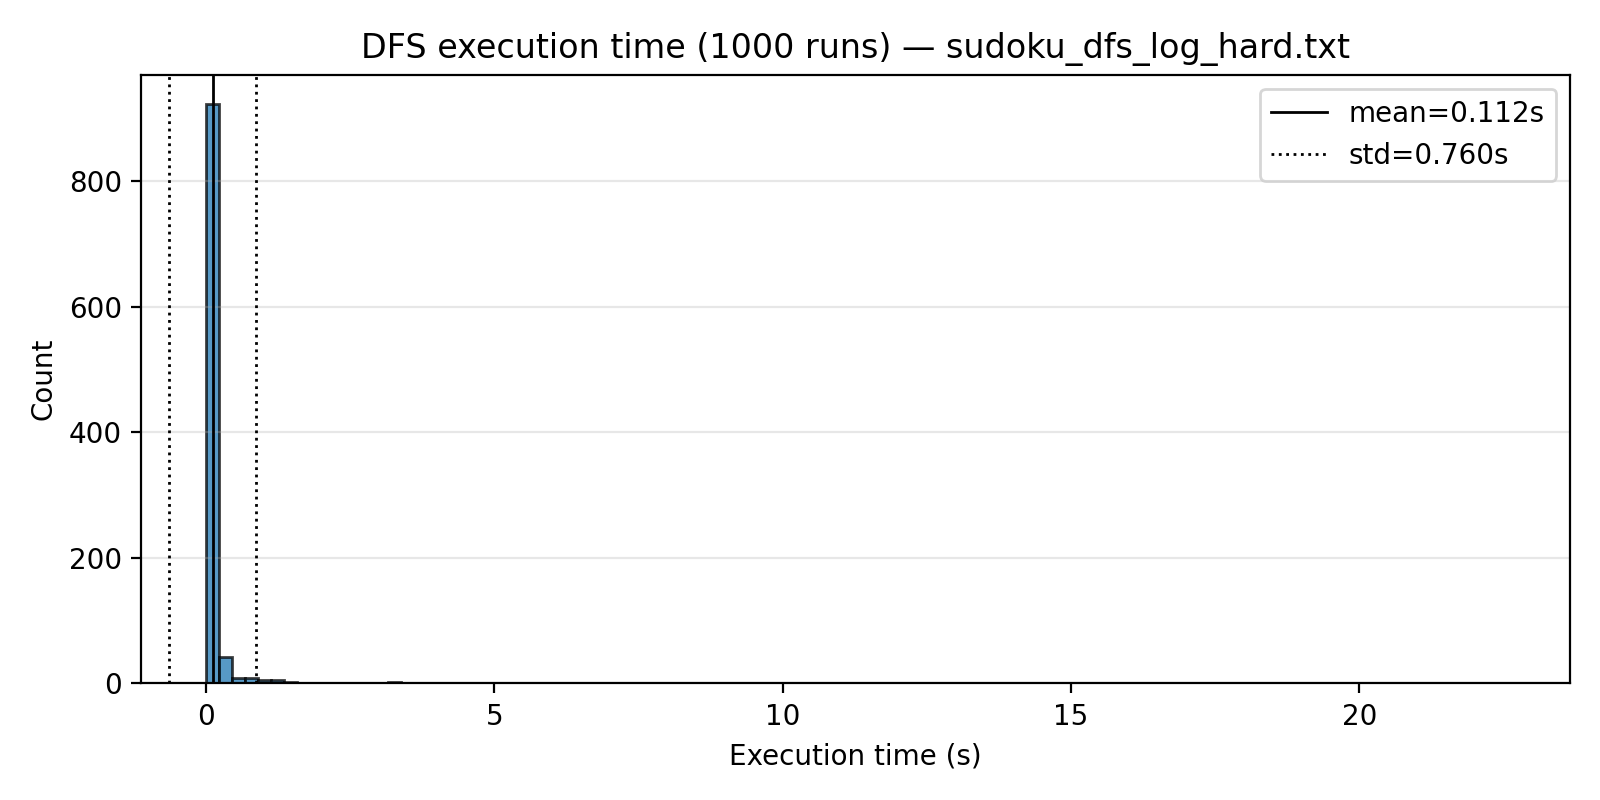
\includegraphics[width=0.8\textwidth]{resources/sudoku_dfs_log_hard_histogram.png}
\caption{sudoku\_dfs\_log\_hard\_histogram.}
\label{fig:sudoku_dfs_log_hard_histogram}
\end{figure}

The charts illustrate that no matter how hard the puzzle is, the rule based algorithm can solve it in a short time. Moreover, the execution time is very stable, only taking 0.001s-0.002s to solve each puzzle. It is immediately apparent that the DFS algorithm drastically outperforms the implemented GA algorithm.
